\subsection[Neumann Zyklus]{Von Neumann Zyklus}
\label{subsec:Neumann-Zyklus}

Der Von Neumann Zyklus der UMach ist auf 4 Schritte verkürzt. Dies ist möglich,
da die Instruktionsbreite immer aus 4 Wörtern besteht, und somit der 
\glqq\textsc{Fetch}\grqq\ von 
Befehl und zugehörigen Operanden in einem gemeinsamen Schritt durchgeführt
werden kann. Somit besteht der Zyklus aus einem beginnenden \textsc{Fetch}. Bei
diesem wird der an der im Programmcounter \texttt{PC} liegende Adresse
gespeicherte Befehl in das Instruktionsregister \texttt{IR} geladen. Danach
wird der im ersten Byte liegende Befehl mit Hilfe des Befehlsdecoders decodiert
und an der ALU entsprechend eingestellt. Danach folgt der dritte Schritt
\textsc{Execute}, in dem die Instruktion ausgeführt wird. Da das Inkrementieren
des Programmcounters \texttt{PC} parallel zum \textsc{Fetch} und \textsc{Decode}
Schritt statt findet, hat dieser Vorgang, im Falle dass der \texttt{PC} im
\textsc{Execute} Schritt überschrieben wird, keine Auswirkung auf den weiteren
Programmablauf. 
Siehe auch Abbildung \ref{fig:Neumann-Zyklus} auf der Seite
\pageref{fig:Neumann-Zyklus}.

Auflistung der Schritte:

\begin{enumerate}
 \item \textsc{Fetch} --
       Holen der Instruktion aus dem Speicher von der Adresse, welche im PC
       vorliegt.
 \item \textsc{Decode} --
       Decodieren des Befehles und Einstellen der ALU.
 \item \textsc{Execute} --
       Auführen des Befehles in der ALU.
 \item Update \texttt{PC} --
       Inkrementieren des \texttt{PC}. Findet parallel zu \textsc{Fetch} und
       \textsc{Decode} statt.
\end{enumerate}

\begin{figure}[h!tp]
 \centering
 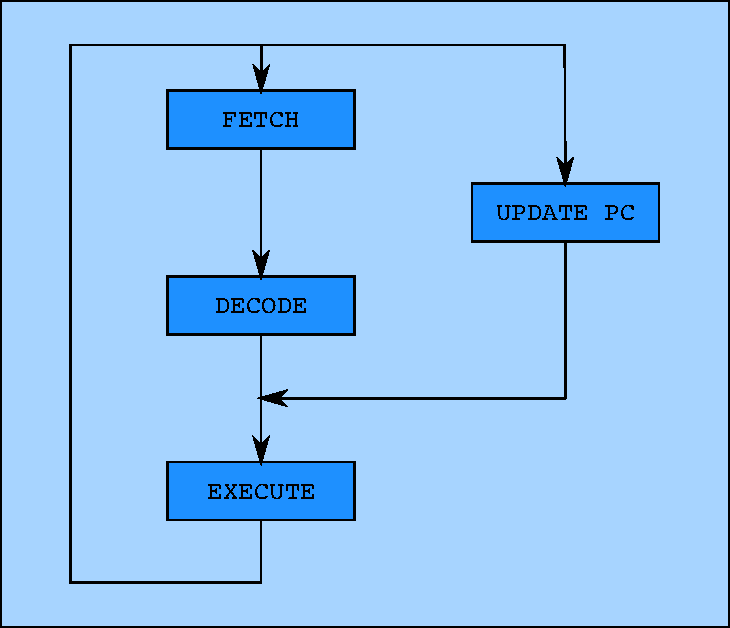
\includegraphics{./img/zyklus.pdf}
 \caption{Von Neumann Zyklus }
 \label{fig:Neumann-Zyklus}
\end{figure}

